\documentclass[10pt,twocolumn,letterpaper]{article}

\usepackage[review]{cvpr}
\usepackage{times}
\usepackage{epsfig}
\usepackage{graphicx}
\usepackage{amsmath}
\usepackage{amssymb}
\usepackage{booktabs}
\usepackage{array}
\usepackage{tabularx}
\usepackage{xcolor}
\usepackage{xspace}

\definecolor{smartblue}{rgb}{0.05,0.25,0.55}

\def\paperID{0000}
\def\confName{CVPR}
\def\confYear{2027}

\newcommand{\smart}{SMART\xspace}
\newcommand{\ours}{SMART-K\xspace}
\newcommand{\exact}{\textsc{Exact}\xspace}
\newcommand{\router}{\textsc{Router}\xspace}

\title{Learning Reusable Geometry Programs for Fast Tight Bounding Box Fitting}

\author{%
Chanhyeok Park\\
SMART Project\\
{\tt\small TODO: affiliation/email}
\and
Minhyuk Sung\\
TODO: affiliation\\
{\tt\small TODO: email}
}

\begin{document}
\maketitle

\begin{abstract}
Split, Merge, and Refine (SMART) fits tight 3D bounding boxes by searching over
box edit actions and evaluating them with an exact geometry reward.  This makes
SMART robust, but the exact Manifold-backed reward dominates runtime because
each refinement or MCTS step can score many candidate edits.  We study a
learning-augmented variant that keeps the exact SMART reward as the final
validator while learning reusable geometry control knowledge.  First, a
set-aware candidate router predicts which one-step edits are worth exact
evaluation, reducing exact reward calls without changing the accepted reward
semantics.  Second, we mine variable-length edit traces into parameterized
macro skills, such as repeated shrink/recenter programs, and validate each
macro with exact rollback-safe execution.  On current local validation pools,
the learned router reduces exact checks by 55.5--79.9\% with zero oracle-regret
turns, guarded learned MCTS improves exact score while using 0.695$\times$ the
wall time on a 309-state pool, and a packaged macro-skill controller improves
mean exact delta from $+1.6118$ to $+1.6639$ on a 173-state replay with
145/28/0 wins/ties/losses against the previous conditional-budget controller.
The results suggest that SMART's large nominal search space contains reusable
3D fitting programs that can be retrieved and verified instead of exhaustively
rescored.
\end{abstract}

\section{Introduction}

Fitting a small set of tight boxes to a 3D shape is useful for interpretable
shape abstraction, collision proxies, scene reasoning, and downstream geometry
processing.  SMART~\cite{park2024smart} approaches this problem by splitting a
shape into over-segmented parts, merging compatible parts, and refining the
resulting boxes through iterative search.  A key strength of SMART is that it
does not rely on a learned cuboid generator.  Candidate edits are accepted
according to an exact geometry objective, so the method remains grounded in the
actual mesh and tetrahedral shape representation.

The same exactness is also the main bottleneck.  At each refinement turn, SMART
enumerates box edit candidates and calls an exact geometry backend to score
them.  MCTS broadens this search to escape local minima, but it further
increases the number of exact reward calls.  The central question in this draft
is therefore:

\begin{quote}
Can we keep exact SMART reward validation, but avoid spending exact geometry
calls on actions that reusable geometry knowledge can already rule out?
\end{quote}

We answer this with two complementary ideas.  The first is a learned candidate
router: a DeepSets-style scorer ranks candidate edits from structured geometry
tokens, after which SMART exact-scores only a guarded top subset.  The model
does not output final boxes and does not replace the reward.  It only changes
which actions are sent to the expensive exact evaluator first.

The second idea is variable-length geometry skills.  Instead of treating every
primitive action independently, we mine successful SMART traces for repeated
programs.  A useful skill is represented by a precondition, a parameterized
edit program, a termination rule, and an exact rollback condition.  This turns
frequent local patterns into reusable control knowledge that can be retrieved
and validated on new states.

\paragraph{Contributions.}
This draft makes four concrete contributions:
\begin{itemize}
\item We formulate SMART acceleration as \emph{exact-reward routing}: learning
predicts which candidates to check, while exact SMART reward still chooses the
accepted edit.
\item We introduce geometry tokens for shape, box, candidate, and history
context, allowing set-aware ranking without learning final cuboids directly.
\item We show that learned priors can make deeper guarded MCTS practical by
reducing wasted exact evaluations.
\item We mine repeated SMART traces into variable-length fitting skills with
preconditions, termination, and rollback, giving an interpretable form of 3D
control knowledge.
\end{itemize}

\begin{figure}[t]
  \centering
  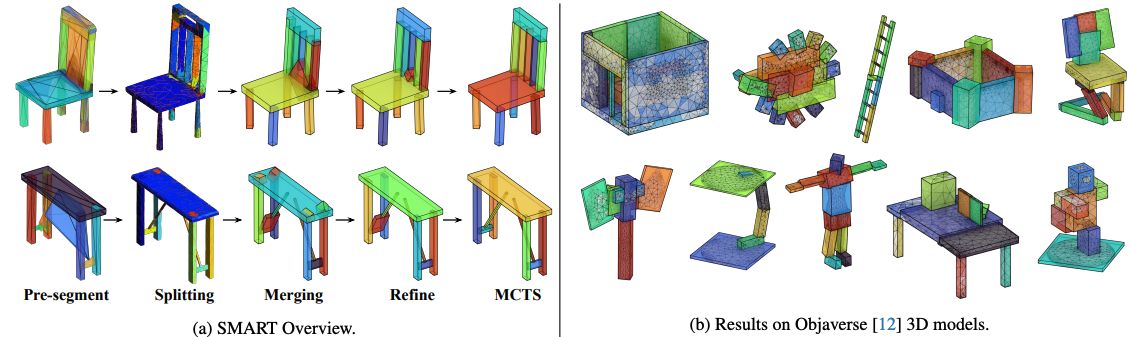
\includegraphics[width=\linewidth]{figures/smart_teaser.png}
  \caption{SMART fits tight boxes through exact geometry-guided search.  This
  draft studies learned routing and reusable macro skills that reduce the
  number of exact candidate evaluations while leaving final acceptance to the
  exact SMART/Manifold reward.}
  \label{fig:teaser}
\end{figure}

\section{Related Work}

\paragraph{Primitive and cuboid abstraction.}
Learning-based primitive abstraction methods generate volumetric primitives or
compact mesh decompositions directly from shape observations
\cite{tulsiani2017learning,chen2020bspnet}.  These methods can be fast at
inference time, but they optimize a learned abstraction objective and can lose
the exact reward semantics required by SMART.  Our goal is different: use
learning to guide the search, while exact geometry remains the acceptance
criterion.

\paragraph{Search and planning.}
MCTS~\cite{kocsis2006bandit} and policy-guided tree search
\cite{silver2018general} show that learned priors can focus expensive search.
SMART's refinement problem has a similar structure: many legal edits exist, but
only a small subset is plausible at a given state.  We therefore use learned
priors for action ordering, top-$K$ filtering, and deeper guarded search.

\paragraph{Options and skills.}
The variable-length skill view is related to hierarchical reinforcement
learning and options: a skill has a precondition, internal policy, and
termination condition.  Here, however, the skill is not accepted by a learned
value alone.  It is replayed against the native SMART engine and accepted only
if the exact reward improves or ties under the configured guard.

\section{Background: SMART Refinement}

Let a shape state contain tetrahedral samples, a set of boxes
$B=\{b_i\}_{i=1}^{N}$, and a finite candidate set
$A(s)=\{a_j\}_{j=1}^{M}$.  Each action edits one box face, axis extent, or
center.  The baseline exact loop computes
\begin{equation}
  a^* = \arg\max_{a_j \in A(s)} R_{\text{exact}}(s, a_j),
\end{equation}
where $R_{\text{exact}}$ is the SMART reward computed by the native
Manifold-backed geometry backend~\cite{huang2020manifoldplus}.  The cost is
proportional to the candidate count times the cost of exact boolean/volume
evaluation.

MCTS expands this into a multi-step search.  It improves local-minimum escape,
but can spend many exact calls on action branches that simple geometry context
would deprioritize.

\section{Method}

\subsection{Geometry Tokenization}

Each refinement turn is converted into structured tokens rather than natural
language.  We use three token families:

\begin{itemize}
\item \textbf{Shape tokens}: category, turn index, number of boxes, current
score summaries, centroid extent, PCA-like extent, and volume histogram
features.
\item \textbf{Box tokens}: center, size, aspect ratio, relative volume,
rotation summaries, and per-box contribution proxies.
\item \textbf{Candidate tokens}: affected box, face/axis, delta, action type,
proxy coverage change, proxy box-volume change, invalidity flags, and
set-aware ranks.
\end{itemize}

Offline data collection exact-scores every candidate with SMART and stores the
exact reward table.  At inference time, only the cheap tokens are built before
the learned router proposes a subset for exact scoring.

\subsection{Set-Aware Candidate Router}

The deployed router is a DeepSets candidate scorer.  For each candidate feature
$x_i$, an MLP $\phi$ produces an embedding $h_i$.  We pool over the candidate
set and score each action with another MLP $\rho$:

\begin{align}
  h_i &= \phi(x_i),\\
  c &= [\mathrm{mean}_i(h_i), \mathrm{max}_i(h_i)],\\
  \ell_i &= \rho([h_i, c]).
\end{align}

The model is trained from exact SMART reward tables with a soft ranking loss:
\begin{equation}
  y_i =
  \frac{\exp((r_i-\max_j r_j)/\tau)}
       {\sum_j \exp((r_j-\max_k r_k)/\tau)}.
\end{equation}
The learned logits $\ell_i$ rank candidates, but the final accepted action is
still chosen by exact scoring among the selected candidates.

\subsection{Guarded Exact Selection}

The router is wrapped in conservative guards:

\begin{enumerate}
\item If a candidate pool is small or ambiguous, score more candidates exactly.
\item For one-box states where model overhead dominates, use the exact native
shortcut.
\item In MCTS, use learned priors to narrow or order branches, but fall back to
exact shallow search on low-confidence states.
\item Every accepted primitive or macro action is validated by
$R_{\text{exact}}$ and can be rolled back.
\end{enumerate}

This design makes the learned component a speed and search-ordering mechanism,
not a new geometric objective.

\begin{figure}[t]
\small
\fbox{\begin{minipage}{0.94\linewidth}
\textbf{Algorithm 1: Guarded exact routing}\\
\textbf{Input:} state $s$, candidates $A(s)$, router $f_\theta$, exact reward
$R_{\text{exact}}$\\
1. Build geometry tokens for all candidates.\\
2. Compute learned scores $\ell_i=f_\theta(s,a_i)$.\\
3. Select a guarded subset $K(s)$ by top-$K$, ambiguity, and fallback rules.\\
4. Evaluate $R_{\text{exact}}(s,a_i)$ only for $a_i \in K(s)$.\\
5. Apply the exact-best candidate in $K(s)$; otherwise rollback/fallback.
\end{minipage}}
\caption{The learned model only reduces the candidate set sent to exact
geometry scoring.  It never directly commits a box edit.}
\label{fig:router_algo}
\end{figure}

\subsection{Variable-Length Geometry Skills}

One-step routing can still be locally myopic.  We therefore mine successful
SMART traces for repeated multi-step programs.  A mined skill is represented as
\begin{equation}
  \mathcal{S} =
  (\text{precondition}, \text{program}, \text{termination}, \text{rollback}).
\end{equation}

For example, a common high-level form is:
\begin{quote}
expand or recenter a box to recover coverage, then repeatedly shrink slack
faces until exact score stops improving.
\end{quote}

In the current implementation, raw traces are canonicalized by replacing
absolute box identifiers with roles, absolute axes with relative geometric
roles, and fixed step counts with repeat predicates where possible.  The first
validated family is a repeated shrink/recenter option.  It is executed by a
live skill controller that tries a small number of macro candidates, validates
them with exact SMART reward, and rolls back failed branches.

\begin{figure}[t]
\small
\fbox{\begin{minipage}{0.94\linewidth}
\textbf{Algorithm 2: Rollback-safe skill execution}\\
\textbf{Input:} state $s$, skill library $\mathcal{L}$, exact reward
$R_{\text{exact}}$\\
1. Retrieve skills whose preconditions match $s$.\\
2. Instantiate each skill's target box/face/axis parameters.\\
3. Execute the internal program until termination or max steps.\\
4. Score the final state with $R_{\text{exact}}$.\\
5. Accept the best non-worse skill; rollback all failed branches.
\end{minipage}}
\caption{A variable-length skill can run for different numbers of primitive
steps on different shapes, but its final update is still exact-validated.}
\label{fig:skill_algo}
\end{figure}

\section{Experiments}

\subsection{Evaluation Protocol}

We report local research validation rather than final benchmark numbers.  The
main metrics are:

\begin{itemize}
\item \textbf{Exact call reduction}: percentage fewer candidate exact scores.
\item \textbf{Wall-time ratio}: learned or skill-guided time divided by exact
baseline time.
\item \textbf{Score change}: final exact SMART score difference.
\item \textbf{Quality losses}: number of states where the learned path is worse
than the exact baseline under the configured comparison.
\end{itemize}

The current draft uses held-out validation pools produced from native SMART
refinement traces, including unseen probe states, mixed category states, hard
airplane multibox states, and one-box live states.  For a final submission, the
split should be frozen before model selection.  In particular, macro-skill
precondition mining should be evaluated on a larger held-out set because rare
failure modes, especially table states with severe upper-repeat failures, are
underrepresented in the current pool.

\begin{table}[t]
\centering
\small
\begin{tabularx}{\linewidth}{lcc}
\toprule
Path & Exact reward final? & Status \\
\midrule
Native SMART refine & yes & release default \\
Learned router refine & yes & opt-in research \\
Guarded learned MCTS & yes & validation-only \\
Variable-length skills & yes & experiment-only \\
Packaged macro-skill controller & yes & opt-in post-refine \\
Direct learned cuboids & no & not used \\
\bottomrule
\end{tabularx}
\caption{All proposed acceleration paths keep exact SMART reward as the final
validator.  The release default remains native exact SMART; learned components
are opt-in or experimental until larger held-out validation is complete.}
\label{tab:status}
\end{table}

\subsection{Same-Turn Candidate Routing}

\begin{table}[t]
\centering
\small
\begin{tabularx}{\linewidth}{lccc}
\toprule
Split & Quality & Exact checks & Speed \\
\midrule
Unseen probe50, 120 states & zero regret & $-67.1\%$ & $1.34\times$ \\
Mixed case41, 39 states & zero regret & $-55.5\%$ & $1.59\times$ \\
Hard airplane, 28 states & zero regret & $-79.9\%$ & $2.02\times$ \\
\bottomrule
\end{tabularx}
\caption{Same-turn router validation.  ``Zero regret'' means the selected
candidate subset still contained an oracle-best action for the evaluated turn.}
\label{tab:router}
\end{table}

Table~\ref{tab:router} shows that a learned router can remove a large fraction
of exact scoring calls while preserving the oracle action on these validation
turns.

\subsection{Budget Reinvestment}

The saved exact-call budget can be reinvested into more refinement turns.  On
hard airplane states, exact 4-turn refinement compared with hard-router 6-turn
refinement improved score by $+0.4010$, used $58.2\%$ fewer exact calls, and was
$18.4\%$ faster with zero losses.  On mixed case41 states, exact 4-turn versus
auto-router 6-turn improved score by $+0.3464$ with $25.1\%$ fewer exact calls
and approximately equal wall time.

\subsection{Guarded Learned MCTS}

\begin{table}[t]
\centering
\small
\begin{tabularx}{\linewidth}{lccc}
\toprule
Setting & Score & Nodes & Speed \\
\midrule
MCTS50 top-$K$ prior & $+0.0139$ & $41.15 \rightarrow 23.74$ & $61.8\%$ faster \\
MCTS50 top-$K$ + TT & $+0.0139$ & $41.15 \rightarrow 22.75$ & $70.6\%$ faster \\
Depth4 frontier + TT & $+0.7121$ & $41.15 \rightarrow 20.52$ & $81.3\%$ faster \\
Guarded pool, 309 states & $+0.7738$ & -- & $0.695\times$ wall \\
\bottomrule
\end{tabularx}
\caption{Learned MCTS prior results.  Aggressive frontier settings are
validation-only; guarded settings retain exact fallback on low-confidence
states.}
\label{tab:mcts}
\end{table}

Learned priors are most useful when they make deeper but narrower MCTS
affordable.  The guarded 309-state pool improved mean exact score and reduced
wall time while recording zero observed losses in the checked pool.

\subsection{Mined Variable-Length Skills}

The strongest current mined pattern is a repeated shrink/recenter family:
\begin{quote}
\texttt{shrink\_face x2 -> recenter\_box x1 -> shrink\_face x7 ->}
\texttt{ recenter\_box x1 -> shrink\_face x2}.
\end{quote}
It is not used as a fixed literal sequence only; variants are grouped into
repeat programs with preconditions.

\begin{table}[t]
\centering
\small
\begin{tabularx}{\linewidth}{lccc}
\toprule
Skill policy & States & Score & Failures \\
\midrule
Median repeat & 176 & $+1.5599$ & 0 \\
Upper repeat, all categories & 176 & $+1.5834$ & 1 \\
Category upper non-table & 176 & $+1.6060$ & 0 \\
Mined conditional upper & 176 & $+1.6146$ & 0 \\
Conservative LCB table-open & 176 & $+1.6200$ & 0 \\
\bottomrule
\end{tabularx}
\caption{Variable-length repeat-skill validation.  The mined conditional rule
uses upper-repeat for airplane/chair and for table only under a learned
geometric precondition.  The conservative LCB rule opens upper-repeat for table
only when the opened training subset has positive lower-confidence-bound gain
and no observed severe loss.}
\label{tab:skills}
\end{table}

Table~\ref{tab:skills} suggests that reusable multi-step skills can outperform
a single median repeat program, but the validation caveat is important:
cross-validation is weaker because severe table failures are rare.  The result
is promising research evidence, not yet a release default.
On a harder chair/table subset biased toward nontrivial first-skill failures,
the same conservative table-open rule improved mean delta from $+1.1002$ to
$+1.1438$ with all $79$ skills accepted, while blind upper-repeat dropped to
$+1.0755$ and lost one case.
On the full hard-state portfolio of $173$ runnable states, the same rule
improves mean delta from $+1.5200$ to $+1.5759$ and keeps all states accepted,
whereas blind upper-repeat accepts $172/173$ states and degrades table mean
delta.

\begin{table}[t]
\centering
\small
\begin{tabularx}{\linewidth}{lccc}
\toprule
Packaged controller & Attempts & Score & W/T/L \\
\midrule
Prior conditional budget & 1.590 & $+1.6060$ & -- \\
Guarded variable repeat & 1.590 & $+1.6118$ & 101/72/0 \\
Quality preset, top-5 exact & 5.000 & $+1.6639$ & 145/28/0 \\
\bottomrule
\end{tabularx}
\caption{Packaged macro-skill controller on the current 173-state replay.
Every accepted update is exact SMART/Manifold non-worse; failed branches are
rolled back.  W/T/L is measured against the prior conditional-budget
controller.}
\label{tab:packaged_macro}
\end{table}

The packaged controller is the safer promotion target than the raw repeat
experiments: it exposes a stable API/CLI, reports its exact-validator and
rollback safety contract, and keeps the release default unchanged.  It should
still be treated as an opt-in post-refinement stage until larger
pipeline-level held-out validation is complete.

\section{Discussion}

\paragraph{Why this is not direct cuboid learning.}
The model does not predict final box geometry.  It predicts which exact
evaluations are likely to matter.  This is why the method can preserve SMART's
reward semantics while still using learning.

\paragraph{Why speed and quality can improve together.}
The router is not only a pruning device.  When exact calls are saved, the same
wall-time budget can be reinvested into additional refine turns or deeper MCTS.
This is why some experiments show both lower runtime and higher final exact
score.  In these cases, the learned model changes the allocation of exact
geometry calls: fewer calls are spent on low-value one-step candidates, and more
calls are spent on later turns or deeper branches that the exact baseline could
not afford under the same budget.
For macro skills, a hybrid program-gate plus macro-memory selector recovers the
current hard-state top-3 exact quality using only two exact skill evaluations,
suggesting that reusable program identity can reduce exact calls without
changing the final validator.  Adding a simple branch-opening precondition
(\eg, open the second exact skill only for under-decomposed table states with
low action count) further reduces the hard-state mean exact skill attempts to
$1.197$ while preserving the top-3 mean delta within $0.00044$.
When quality is prioritized over maximum pruning, a conditional exact-budget
ladder chooses one, two, or three exact skill checks from category or bbox
statistics.  On a runnable 133-state portfolio, the rule
\emph{airplane: one check, chair: two checks, table: three checks} recovers
top-3 quality within $0.0010$ mean delta while reducing exact skill attempts
from $3.000$ to $1.669$.

\paragraph{What counts as 3D knowledge.}
The extracted knowledge is a programmatic control structure: preconditions,
parameterized edits, termination, and rollback.  This is more reusable than a
literal action string because the same skill can run for a variable number of
steps depending on coverage and slack predicates.

\paragraph{Can this reach global optima?}
No finite learned skill library guarantees global optimality for the full SMART
search space.  However, it can approximate the useful part of MCTS: escaping
local minima by trying structured multi-step programs instead of enumerating a
large tree blindly.  Exact validation remains the safety mechanism.

\section{Reproducibility}

The implementation is organized as an opt-in research path on top of the
released native SMART package.  The baseline release path remains exact native
SMART.  The learned experiments use the following artifacts:

\begin{itemize}
\item native C++ SMART engine for exact action scoring and rollback,
\item offline candidate-token collectors that store exact reward tables,
\item a packaged DeepSets router checkpoint for one-step candidate ranking,
\item MCTS prior wrappers that convert router scores into action priors,
\item macro-skill miners and live executors in the experiment tree.
\end{itemize}

The main experiment families can be reproduced from the repository with:

\begin{quote}
\small
\texttt{collect\_live\_geometry\_policy\_tokens.py}\\
\texttt{train\_deepset\_candidate\_scorer.py}\\
\texttt{evaluate\_native\_deepset\_engine\_policy.py}\\
\texttt{evaluate\_deepset\_mcts\_prior.py}\\
\texttt{evaluate\_live\_skill\_controller.py}
\end{quote}

For a submission version, these scripts should be wrapped in a frozen benchmark
manifest so that train, validation, and test states are not mixed during model
selection.

\section{Ablations}

Several negative or weaker results are important for interpreting the method.
First, one-box states often do not benefit from neural routing because the
candidate pool is already small; the portfolio therefore keeps them on the
exact native shortcut.  Second, aggressive top-1 MCTS pruning can be very fast
but is unsafe on low-confidence multibox states, so the guarded configuration
falls back to exact shallow search for those states.  Third, a simple MLP gate
for choosing repeat programs was weaker than mined conditional rules on the
current data.  This suggests that the useful abstraction is not merely a binary
classifier, but a preconditioned variable-length program with explicit rollback.

\section{Limitations and Next Steps}

The current evidence is local and should be expanded before a paper claim is
finalized.  The next experiments should:

\begin{itemize}
\item increase held-out category and shape coverage,
\item report full train/validation/test splits for router and skill mining,
\item integrate the skill executor more deeply into the native C++ engine,
\item train a transformer-style skill retrieval model over shape, box,
candidate, and history tokens,
\item compare against fixed-budget MCTS and exact refine on full pipeline
outputs, not only refinement states.
\end{itemize}

\section{Conclusion}

SMART's expensive exact geometry reward is reliable but overused.  This draft
shows that learned routing and mined variable-length skills can reduce exact
calls and sometimes improve final score by spending search budget more
intelligently.  The most important design constraint is that exact
SMART/Manifold reward remains the final validator.  Under that constraint,
learning becomes a reusable geometry-control layer rather than an approximate
replacement for SMART.

{\small
\bibliographystyle{ieeenat_fullname}
\bibliography{refs}
}

\end{document}
